\documentclass[letterpaper,10pt]{article}

\usepackage{titling}
\usepackage{listings}
\usepackage{url}
\usepackage{setspace}
\usepackage{subfig}
\usepackage{sectsty}
\usepackage{pdfpages}
\usepackage{colortbl}
\usepackage{multirow}
\usepackage{relsize}
\usepackage{amsmath}
\usepackage{fancyvrb}
\usepackage{amsmath,amssymb,amsthm,graphicx,xspace}
\usepackage[titlenotnumbered,noend,noline]{algorithm2e}
\usepackage[compact]{titlesec}
\usepackage{paratype} 
\usepackage[T1]{fontenc}
\usepackage{tikz}
\usetikzlibrary{arrows,automata,shapes,trees,matrix,chains,scopes,positioning,calc}
\tikzstyle{block} = [rectangle, draw, fill=blue!20, 
    text width=2.5em, text centered, rounded corners, minimum height=2em]
\tikzstyle{bw} = [rectangle, draw, fill=blue!20, 
    text width=4em, text centered, rounded corners, minimum height=2em]

\definecolor{namerow}{cmyk}{.40,.40,.40,.40}
\definecolor{namecol}{cmyk}{.40,.40,.40,.40}

\let\LaTeXtitle\title
\renewcommand{\title}[1]{\LaTeXtitle{\textsf{#1}}}


\newcommand{\handout}[5]{
  \noindent
  \begin{center}
  \framebox{
    \vbox{
      \hbox to 5.78in { {\bf ECE254: Operating Systems and Systems Programming } \hfill #2 }
      \vspace{4mm}
      \hbox to 5.78in { {\Large \hfill #4  \hfill} }
      \vspace{2mm}
      \hbox to 5.78in { {\em #3 \hfill} }
    }
  }
  \end{center}
  \vspace*{4mm}
}

\newcommand{\lecture}[3]{\handout{#1}{#2}{#3}{Lecture #1}}
\newcommand{\tuple}[1]{\ensuremath{\left\langle #1 \right\rangle}\xspace}

\addtolength{\oddsidemargin}{-1.000in}
\addtolength{\evensidemargin}{-0.500in}
\addtolength{\textwidth}{2.0in}
\addtolength{\topmargin}{-1.000in}
\addtolength{\textheight}{1.75in}
\addtolength{\parskip}{\baselineskip}
\setlength{\parindent}{0in}
\renewcommand{\baselinestretch}{1.5}
\newcommand{\term}{Spring 2015}

\singlespace


\begin{document}

\lecture{ 10 --- Symmetric Multiprocessing (SMP) }{\term}{Jeff Zarnett}

\section*{Multiprocessing}

Not that long ago, a typical computer had one processor with one core. It could accordingly do exactly one thing at a time. When we say there is one processor, it's one general purpose processor that executes user processes. There may be additional special-purpose processors in the system (e.g., a RAID controller\footnote{The graphics card seems like a more obvious example, but these days there are various programs that can make use of the powerful GPU to do general purpose computation.}) but there is only one general purpose processor so we call it a uniprocessor system.

Now, desktops, laptops, and even cell phones are almost certainly using multi-core processors. A quad-core processor may be executing four different instructions from four different threads at the same time. In theory, multiple processors may mean that we can get more work done in the same amount of (wall clock) time, but this is not a guarantee. Plus, if one of the CPUs in a two-CPU system fails, the system can likely carry on at a reduced performance level.

Multiple processor systems may be \textit{asymmetric multiprocessing} systems or \textit{symmetric multiprocessing} systems. If they are asymmetric, then there is a \textit{boss} processor that is in charge of controlling the system: all other processors are \textit{workers} and they take instructions from the boss or have a very specific task to perform. The other kind of system, symmetric, is more collectivist: the workers are in charge and all processors are equal, comrade!\footnote{History lesson: this idea did not work out so well for the Soviet Union.} Most of the systems we are familiar with (laptops, phones, etc) are symmetric multiprocessing (SMP), but in theory whether a system is symmetric or asymmetric can be configured in software; SunOS version 4 was asymmetric but version 5 (Solaris) is symmetric on the same hardware~\cite{osc}.


A formal definition of SMP, according to~\cite{osi}, is: a stand-alone computer system with the characteristics:
\begin{enumerate}
	\item There are two or more general purpose processors.
	\item The processors share the same main memory and I/O devices and are interconnected by a bus.
	\item All processors are capable of performing the same functions.
	\item The system is controlled by an OS that provides interaction between processors and their programs.
\end{enumerate}

A system with three processors with three processors may be organized something like the diagram below:

\begin{center}
	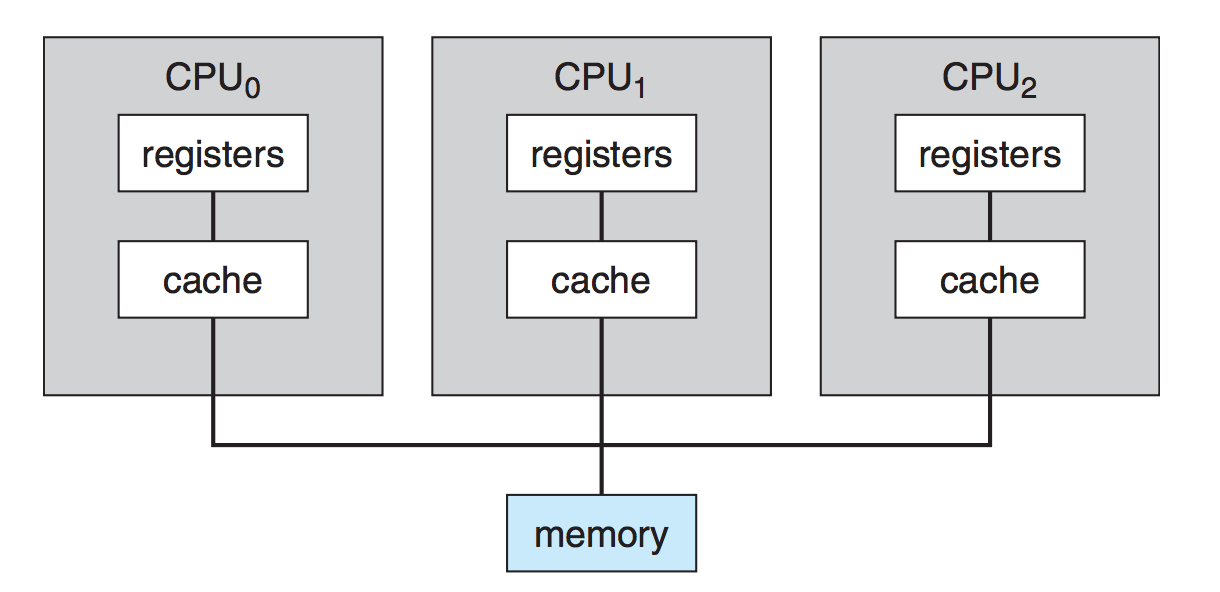
\includegraphics[width=0.5\textwidth]{images/smp-architecture.png}\\
	Symmetric multiprocessing architecture~\cite{osc}.
\end{center}

Terminology note: we often refer to a logical processing unit as a \textit{core}. The term CPU may refer to a physical chip that contains one or more logical processing units. As far as the operating system is concerned, it does not much matter if a system has four cores in four physical chips or four cores in one chip; either way, there are four units that can execute instructions.

If there is exactly one process with one thread running in the system, then it does not matter how many cores are available: at most one core will be used to execute this task. If there are multiple processes, each process can execute on a different core. But what do we do if there are more processes and threads than available cores? We can hope that the processes get blocked frequently enough and long enough so that all processes get to run, but this is not something we can count on.

Our solution is that the CPU should switch between the different tasks via a procedure we call \textit{time slicing}. So thread 1 would execute for a designated period, such as 20 ms, then thread 2 for 20 ms, then thread 3 for 20 ms, then back to thread 1 for 20 ms. To the user, it seems like threads 1, 2, and 3 are being executed in parallel, because 20 ms is fast enough that the user does not notice the difference.

\begin{center}
	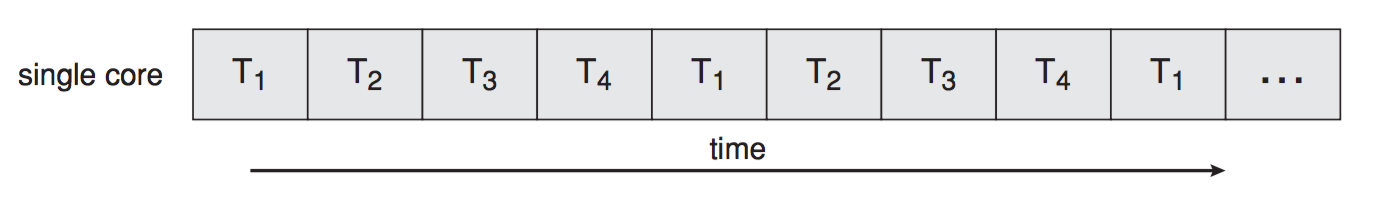
\includegraphics[width=0.7\textwidth]{images/single-core-execution.png}\\
	Execution of different Threads $T_{1}$ through $T_{4}$ on a single core~\cite{osc}.
\end{center}

Time slicing of execution will still occur, if necessary. Continuing our example, if there are four threads running on a dual-core system, time slicing is necessary to run all those programs.

\begin{center}
	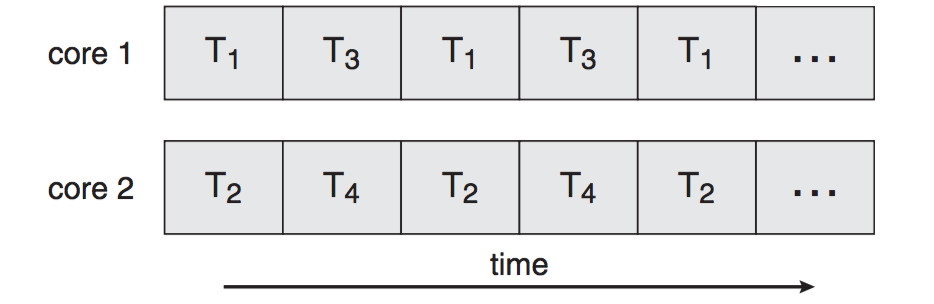
\includegraphics[width=0.7\textwidth]{images/dual-core-execution.png}\\
	Execution of different Threads $T_{1}$ through $T_{4}$ on two cores~\cite{osc}.
\end{center}

The subject of time slicing is something we will return to later on in our discussion of scheduling. 

\subsection*{Parallelism and Speedup}

No doubt it has occurred to you that if there are multiple threads running at the same time, it means a task will get completed faster, right? Well... maybe. It depends a lot on what the task is. There is some overhead involved in splitting a task up and re-combining the results (if necessary), but in most circumstances the overhead is negligible compared to the amount of time working on the task.  

If a task can be fully parallelized, it means the task can be split up in such a way that adding a second executing thread would double the speed of execution. Imagine painting an apartment. It would take one person 12 hours to paint the whole apartment and two people could complete the job in 6 hours. The pattern continues: three people can complete the job in 4 hours, four people in 3 hours, et cetera. This is the ideal, but in the real world there will be a limit to how many additional workers you can add and continue to have this speedup characteristic. At some point, the overhead of adding more threads is no longer negligible. In theory, you could hire 720 painters and finish the job in 1 minute, but at some point you cannot physically fit any more painters into the room.

If a task can be partially parallelized, it means the task can be divided, but doubling the workers doesn't result in completing the job in half the time. Two chefs working together in a kitchen might take 75\% of the time it would take one chef to cook a meal. Adding the extra worker to the kitchen improved the speed at which food was prepared, but it's not doubled. The chefs can work independently some of the time, but at other times one has to wait for the other; the sauce cannot be put on the chicken until the chicken comes out of the oven.

If a task cannot be parallelized at all, then no amount of extra workers will speed it up. Some tasks can only be done sequentially. As the folk saying goes, ``Nine women can't have a baby in one month.''

Let us consider an example from~\cite{mte241}: Suppose we have a task that can be executed in 5~s and this task contains a loop that can be parallelized. Let us also say initialization and recombination code in this routine requires 400~ms. So with one processor executing, it would take about 4.6~s to execute the loop. If we split it up and execute on two processors it will take about 2.3~s to execute the loop. Add to that the setup and cleanup time of 0.4~s and we get a total time of 2.7~s. Completing the task in 2.7~s rather than 5~s represents a speedup of about~46\%.

A smart fellow by the name of Gene Amdahl came up with a formula for the general case of how much faster a task can be completed based on how many processors we have available. Let us define $S$ as the portion of the application that must be performed serially and $N$ as the number of processing cores available. Amdahl's Law:

\begin{center}
speedup $\leq$ {\huge $\frac{1}{S + \frac{1-S}{N}}$}
\end{center}

This is a math formula, after all, and you can do things like take the limit as $N$ approaches infinity and you will find the speedup converges to $\frac{1}{S}$. So the limiting factor on how much additional processors help is, of course, the size of the $S$ term in the equation. That squares well with our intuition about how this should work. If the task is completely sequential (cannot be parallelized at all), we cannot make it faster and $\frac{1}{1 + 0}$ will produce a maximum speedup of 1; or in other words... no speedup at all.

Applying this formula to the example from earlier, we get the following run times:

\begin{center}
	\begin{tabular}{l|l}
	\textbf{Processors} & \textbf{Run Time (s)} \\ \hline
	1 & 5\\
	2 & 2.7\\
	4 & 1.55\\
	8 & 0.975\\
	16 & 0.6875 \\
	32 & 0.54375 \\
	64 & 0.471875 \\
	128 & 0.4359375\\
	\end{tabular}
\end{center}

There are two observations from this data immediately. The first is that we get diminishing returns as we add more processors. Going from 1 to 2 processors reduced the runtime dramatically, but going from 64 to 128 reduced the run time only a very small amount. The second is that as we continue to add more processors we are converging on a run time of 0.4~s, which fits our expectations of what would happen with infinite processors. The serial part will take 0.4~s no matter what, and with infinite processors the parallel part would be (effectively) instant. Again, applying the formula, the most we could speed up this code is by a factor of $\frac{5}{0.4}\approx 12.5$. It is not possible to do better than this. In reality we will never be able to equal the limit either, because nobody has infinite processors available, considering that would take an infinite amount of space and an infinite amount of money...

\subsection*{Merge Sort Example}
Recall from data structures and algorithms the concept of merge sort. This is a divide-and-conquer algorithm like binary search. Split the array of values up into smaller pieces, sort those, and then merge the smaller pieces together to have sorted data. To get this done, we might have many threads sorting and one thread merging the sorted lists together into a larger, sorted list. Visually, this looks like:

\begin{center}
	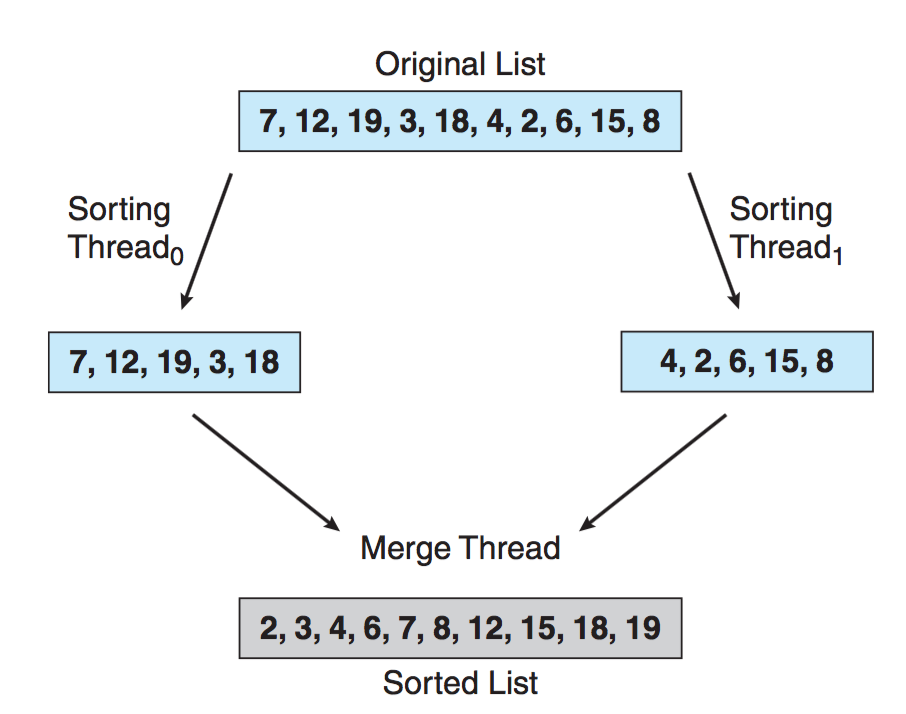
\includegraphics[width=0.55\textwidth]{images/multithread-sort.png}\\
	Multithreaded sorting~\cite{osc}.
\end{center}

In your earlier examination of sorting, you may have learned that for a small array, perhaps of 30 entries or fewer, it makes sense to use one of the simple algorithms like insertion sort (despite $\Theta(n^{2})$ worst-case runtime). Below this threshold, it is more efficient to execute the insertion sort algorithm than it would be to divide up the problem into smaller pieces and recombine those results~\cite{mte241}. You may have seen something similar in optimized binary search algorithms where, at some point, a linear search is used. So let us begin with the code for the insertion sort routine that we will rely upon. This code, and all code in this section, comes from~\cite{mte241}:

\begin{verbatim}
void insertion_sort( double *array, size_t a, size_t b ) {
  size_t j, k;
  double tmp;
  for ( int k = a + 1; k < b; ++k ) { 
    tmp = array[k];
    
    for ( int j = k; j > a; --j ) {
      if ( array[j - 1] > tmp ) {
        array[j] = array[j - 1];
      } else {
        array[j] = tmp;
        break;
      }
    }
    if ( tmp < array[a] ) {
      array[a] = tmp;
    }
  } 
}
\end{verbatim}

So our merge sort algorithm will look like this: if the list is below a certain size, perform the insertion sort. Otherwise, divide the list in half and call merge sort recursively on each half, and then merge the results of those two lists. Merging is a operation all its own, so let us extract that into its own function:

\begin{verbatim}
#include <assert.h>

// Merge the entries from a to b - 1 and from b to c - 1 
void merge( double *array, size_t a, size_t b, size_t c ) {
  assert( a <= b && b <= c );
  
  size_t i = 0, j = a, k = b;
  double *sorted_array = (double *) malloc( (c - a)*sizeof( double ) );
  
  while ( j < b && k < c ) {
    if ( array[j] <= array[k] ) {
      sorted_array[i] = array[j];
      ++j; 
    } else {
      sorted_array[i] = array[k];
      ++k; 
    }
    
    ++i; 
    }
    
  for ( ; j < b; ++i, ++j ) {
    sorted_array[i] = array[j];
  }
    
  for ( ; k < c; ++i, ++k ) {
    sorted_array[i] = array[k];
  }
    
  for ( i = 0, k = a; k < c; ++i, ++k ) {
    array[k] = sorted_array[i];
  }
    
  free( sorted_array );
}
\end{verbatim}

And now we can implement merge sort (which is presently configured such that insertion sort will be used if the array to be examined is smaller than 30 entries).

\begin{verbatim}
#define USE_INSERTION_SORT 30

void merge_sort( double *array, size_t a, size_t c ) {
  assert( a <= c );
  
  if ( c - a < USE_INSERTION_SORT ) {
    insertion_sort( array, a, c );
    return;
  }
  size_t b = a + (c - a)/2;
  
  merge_sort( array, a, b );
  merge_sort( array, b, c );
  merge( array, a, b, c );
}
\end{verbatim}

To run this as a new thread, as you will recall from earlier, we can pass in only one argument for the parameters to the sort function. So we need a \texttt{struct} object to contain the arguments:

\begin{verbatim}
typedef struct interval {
  double *array;
  size_t a;
  size_t c;
} interval_t;
\end{verbatim}

The user does not know that we are going to use a parallel algorithm so the function call should seem somewhat more ``natural'' and delegate to our internal function: 

\begin{verbatim}
void merge_sort( double *array, size_t n ) {
  interval_t arg;
  arg.array = array;
  arg.a = 0;
  arg.c = n;
  merge_sort_internal( &arg );
}

void *merge_sort_interal( void *void_arg ) {
  // the argument is an arbitrary pointer
  //   cast it to a pointer to an instance of 'interval_t'
  interval_t *arg = (interval_t *)void_arg;
  if ( ( arg->c - arg->a ) < USE_INSERTION_SORT ) {
    insertion_sort( arg->array, arg->a, arg->c );
    return NULL;
  }
  
  size_t b = arg->a + (arg->c - arg->a)/2;
  
  interval_t arg1, arg2;
  
  arg1.array = arg->array;
  arg1.a = arg->a;
  arg1.c = b;
  
  arg2.array = arg->array;
  arg2.a = b;
  arg2.c = arg->c;
  
  pthread_t other_thread;

  // Create a thread to sort the second half
  pthread_create( &other_thread, NULL, merge_sort_interal, &arg2 ); 
  merge_sort_interal( &arg1 );
  
  // Wait for them to finish
  pthread_join( other_thread, NULL );

  merge( arg->array, arg->a, b, arg->c );

  return NULL;
}
\end{verbatim}

The execution of this code on an array of capacity 21 and with the insertion sort threshold lowered to 5, when represented visually, looks like this:

\begin{center}
	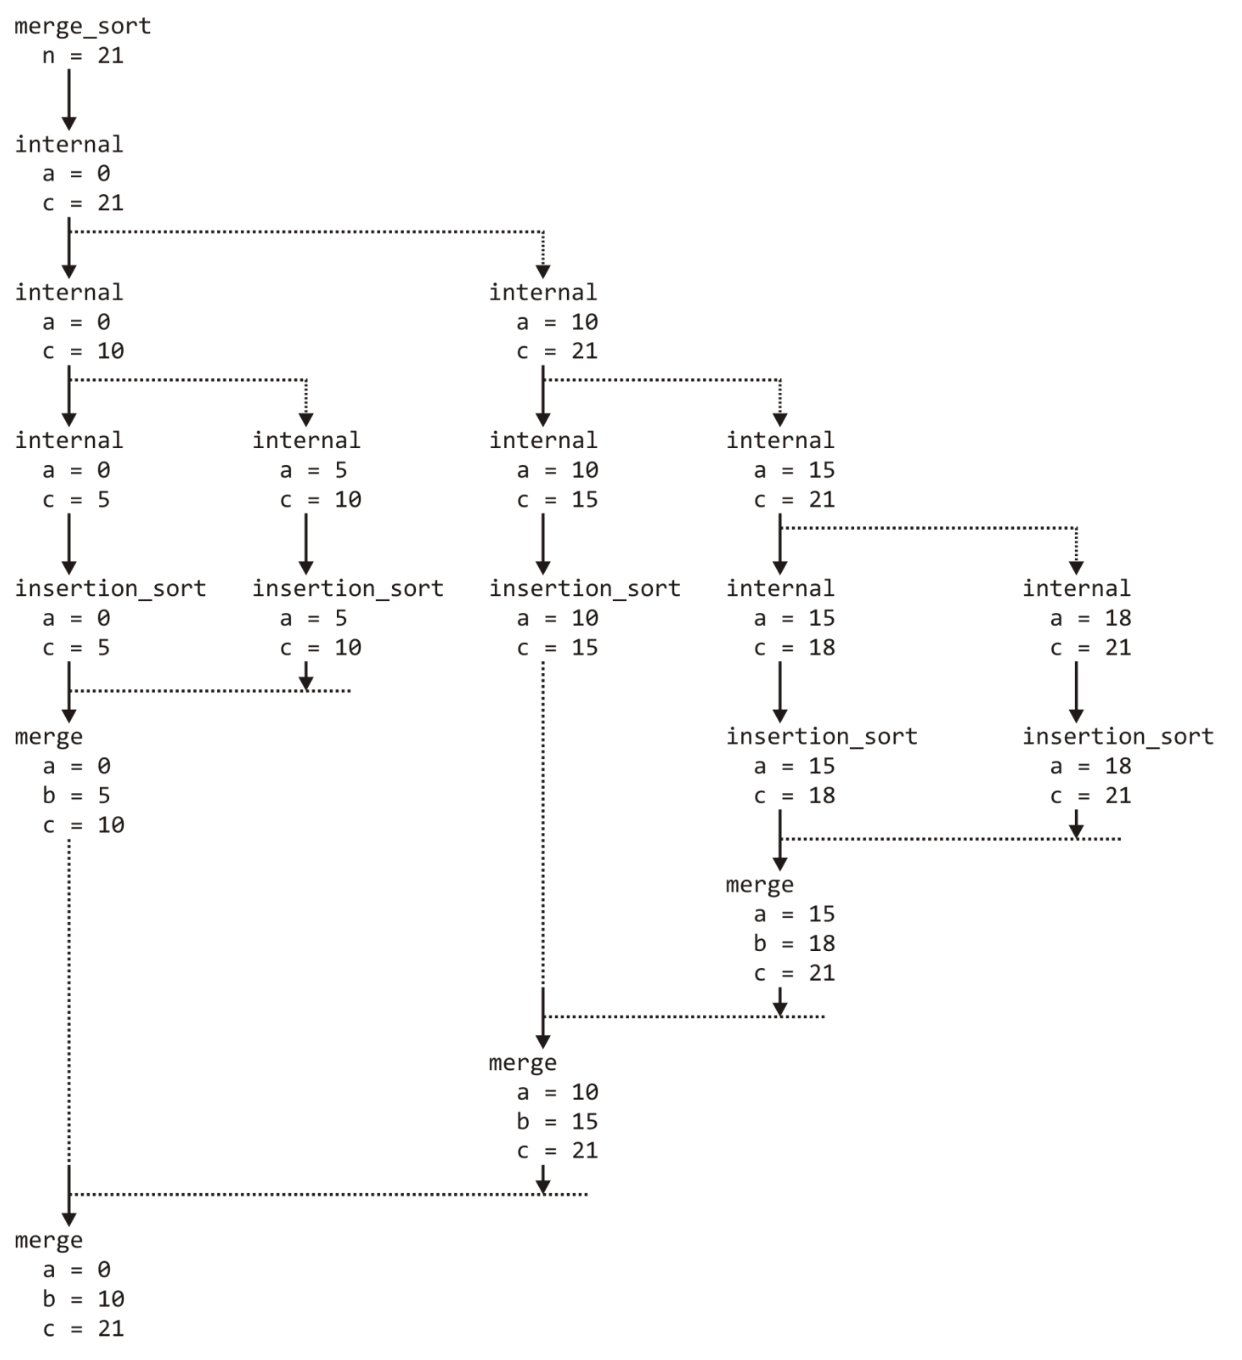
\includegraphics[width=\textwidth]{images/merge-sort-execution.png}\\
	Multithreaded sorting execution in parallel~\cite{mte241}.
\end{center}

The runtime of merge sort, according to the data structures and algorithms course is $\Theta(n$ ln$(n))$; however, if each of the threads execute on their own core, then the run time will be reduced to $\Theta(n)$.

\bibliographystyle{alpha}
\bibliography{254}


\end{document}
